
\section{Introduction}

In recent human history there has been tremendous progress in sciences and the benefits can be coupled with the increase in life expectancy. About 150 years ago an average person would live up to 30 years, but now we're expecting to reach an average age of 70 years, and better prospects are in high-income countries like U.K. or Japan, as seen in Figure \ref{fig:life_expectancy}. Most of the technologies played a role in the increased welfare of the world population, but the advances in healthcare and our biological understanding had directly improved life expectancy. As cancer is typically a disease of ageing and as the world's population grows older a side effect is that more people get cancer in modern times.

In an article titled "Is the world making progress against cancer?"\cite{World_in_Data_undated-gc}\footnote{I found the graphs from Our World in Data to be useful in understanding the scale of cancer and they have more graphs dedicated to cancer on their website\cite{Roser2015-qb}. }, Dr Max Roser gives an overview of humanity's progress on the disease. It is expected, that as both the population and life expectancy grow, there will be more people predisposed to cancers, and this is represented by the green line in Figure \ref{fig:cancer_death}; the cancer death rate increased to 66\% in 2017 from 1990. The red line is the cancer death rate per 100,000 and that only increased 17\% which means that if the World's population will have they stayed the same as in 1990, the cancer deaths will increase only a quarter. If the age is standardized then it can be seen that the death rate drops to -15\%. Therefore, Figure \ref{fig:cancer_death} tells us that there has been some progress in solving cancer, but there is a need for more concentration of effort as life expectancy continues to increase.

\begin{figure}[!htb]
    \centering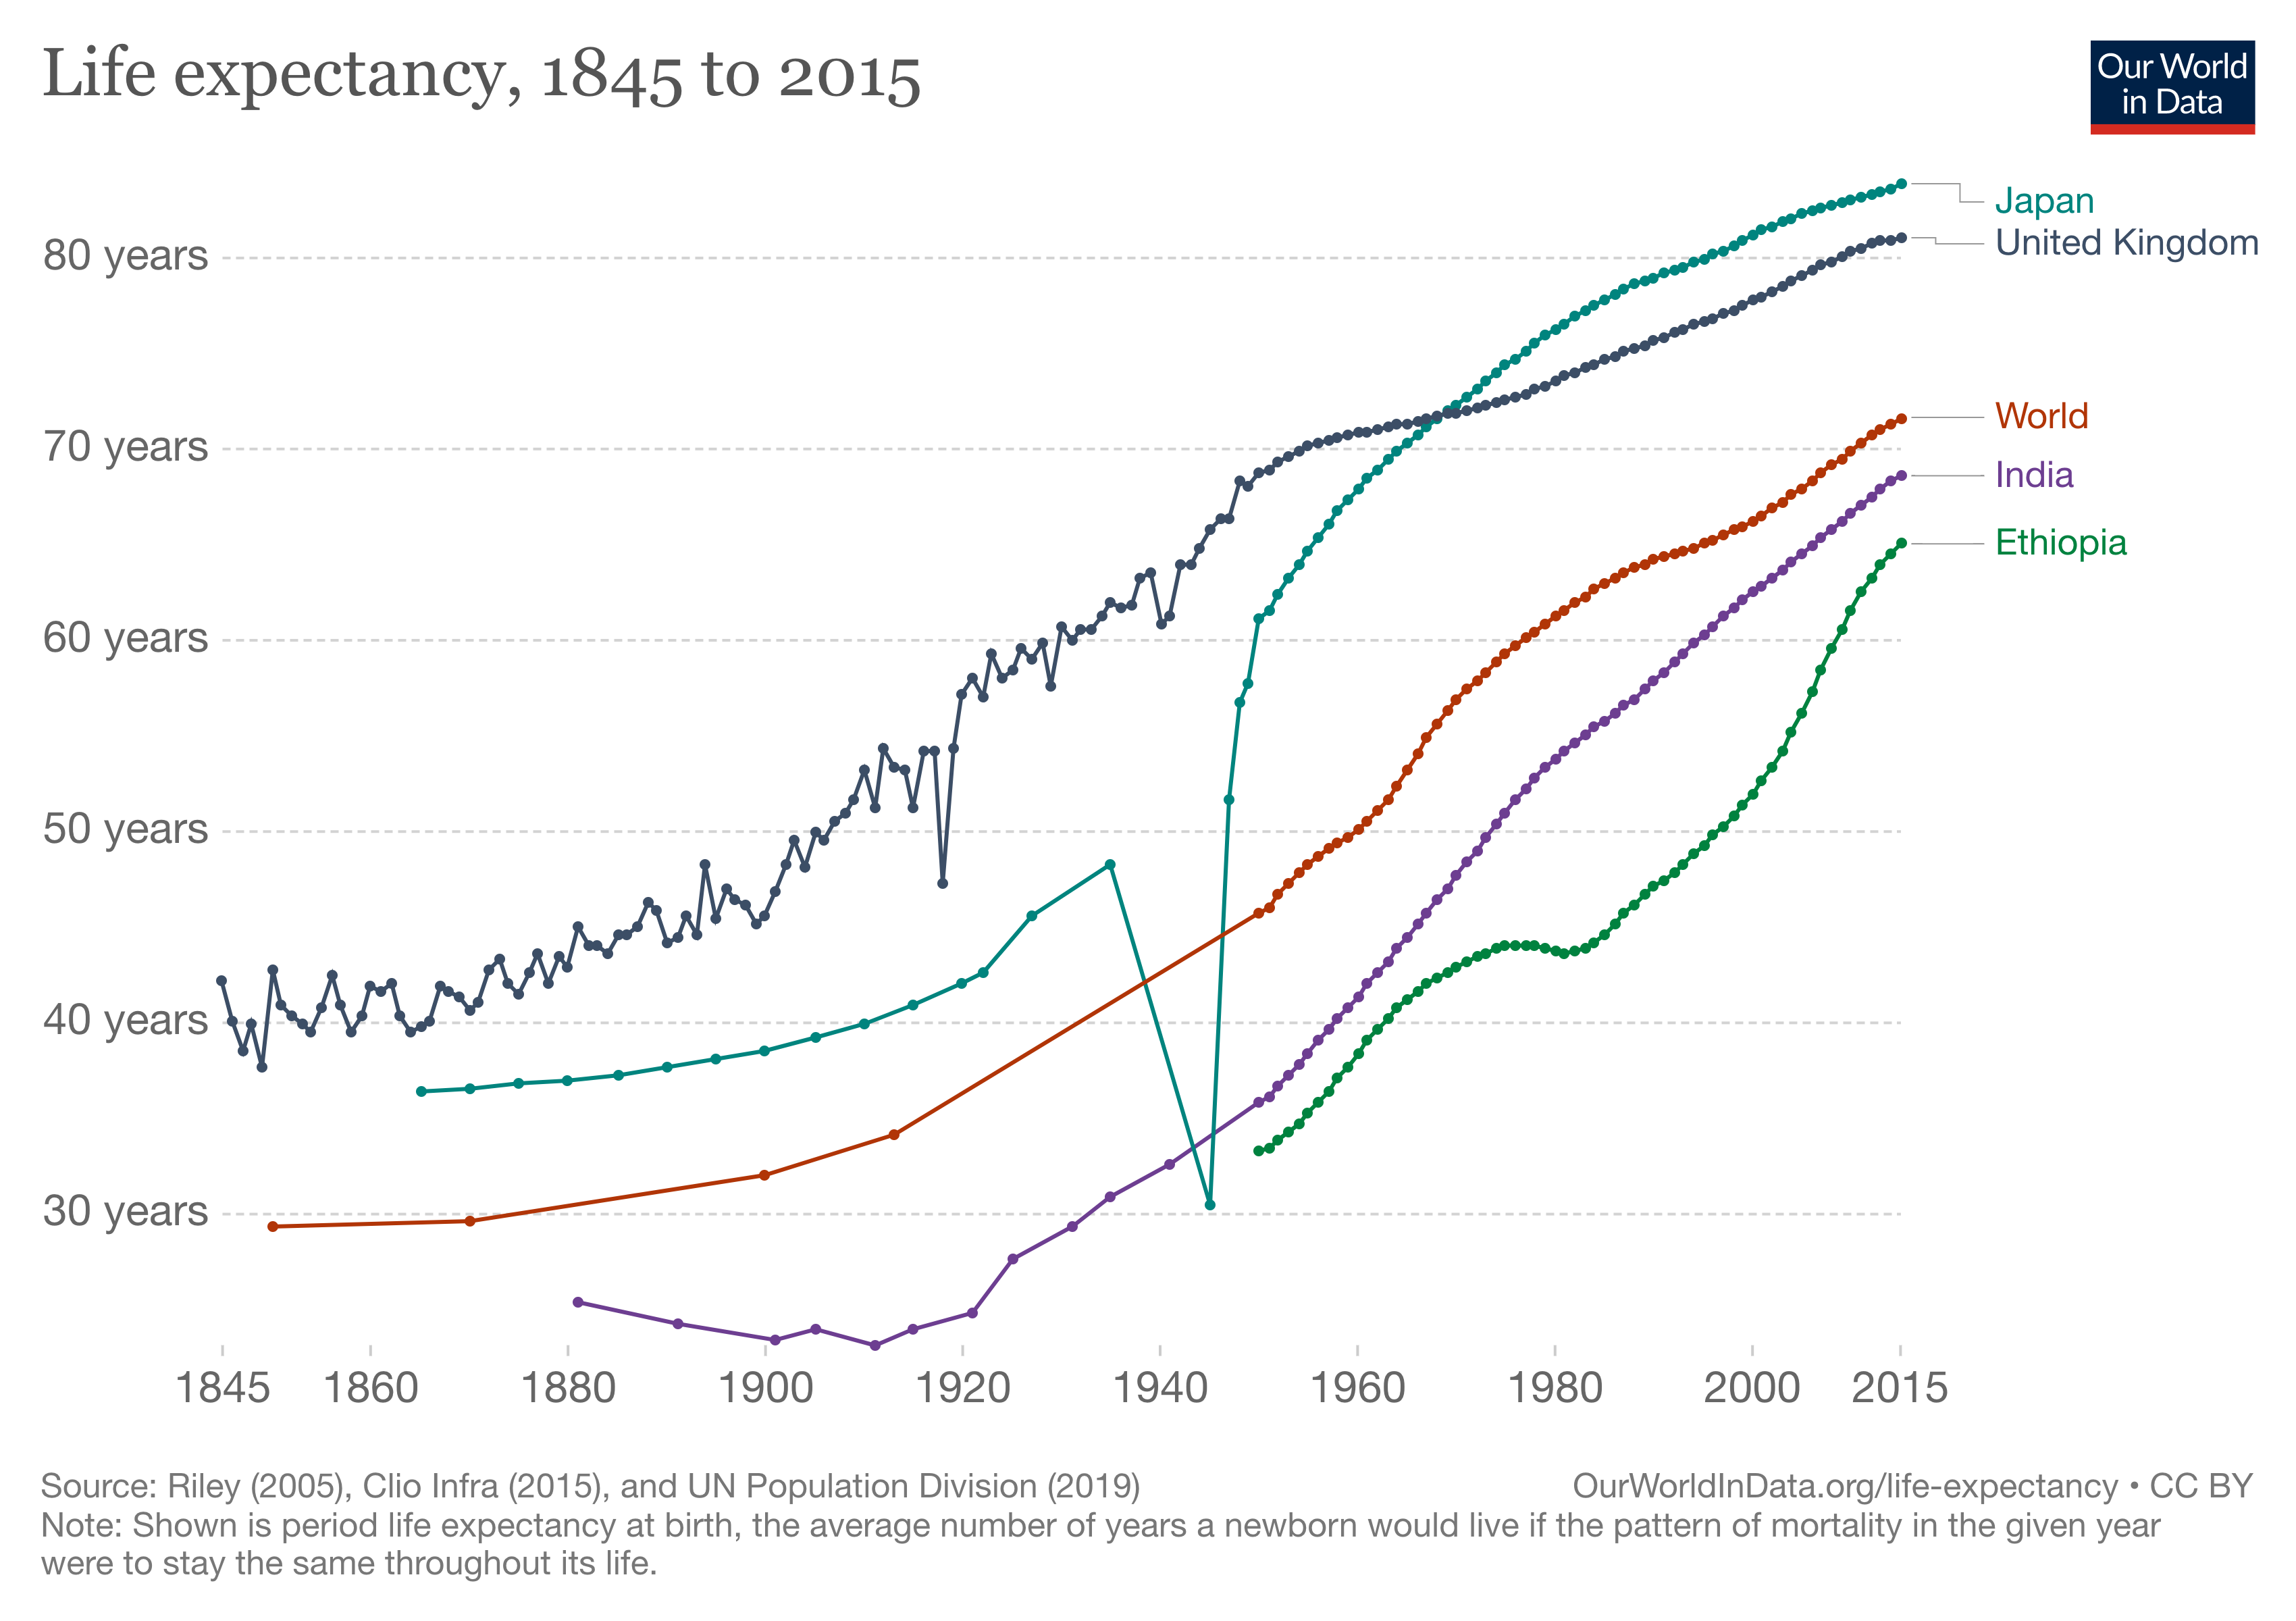
\includegraphics[width=1.0\textwidth,height=0.3\textheight,keepaspectratio]{Images/Resources/life-expectancy.png}
      \caption{Life expectancy according to World in Data between 1845 - 2015\cite{World_in_Data_undated-no}}
      \label{fig:life_expectancy}
  \end{figure}
  \FloatBarrier

According to Cancer Research UK\cite{Cancer_Research_UK2015-cf}, the bladder is the 10th leading cause of death, it accounts for 3\% of all deaths in the U.K. and 56\% of incidence is in people older than 75. Almost half (52.6\%) of the people diagnosed with bladder cancer survive for more than five years, and 46.4\% for more than ten years. 

This project focuses on understanding better the mechanism of cancer from genomic data, which includes both mutation and gene expression. The initial focus will be on bladder cancer as the Jack Birch Unit (JBU) holds knowledge on the normal behaviour of the tissue which enables the integration of domain knowledge into the computational models. Furthermore, there are publicly available datasets on Bladder Cancer such as \acrfull{tcga}\cite{Tcga2018-sj} and Uromol dataset\cite{Lindskrog2021-ov, The_European_Genome-phenome_Archive_undated-pz}.

The purpose of this report is to introduce the reader to the research in multi-omics (Chapter \ref{s:multi-omics}) which itself can be split in multiple areas: Consensus subtyping \& the user of Transcriptomic data (Section \ref{s:rnaSeq}), processing mutations data (Section \ref{s:mutations}), combined approaches (Section \ref{s:multi-view}) and Deep Learning (\ref{s:dl_genomics}). The relevant concepts throughout  Chapter \ref{s:multi-omics} are described in the subsections from Chapter \ref{s:computational}. This document finishes with a discussion and the Aims \& Goals (\ref{s:aims}) of the project, followed by the Risks \ref{s:risks}. In addition, as part of the submission, a Gantt chart is included that describes the project's plan for the upcoming year. 

\begin{figure}[!htb]
    \centering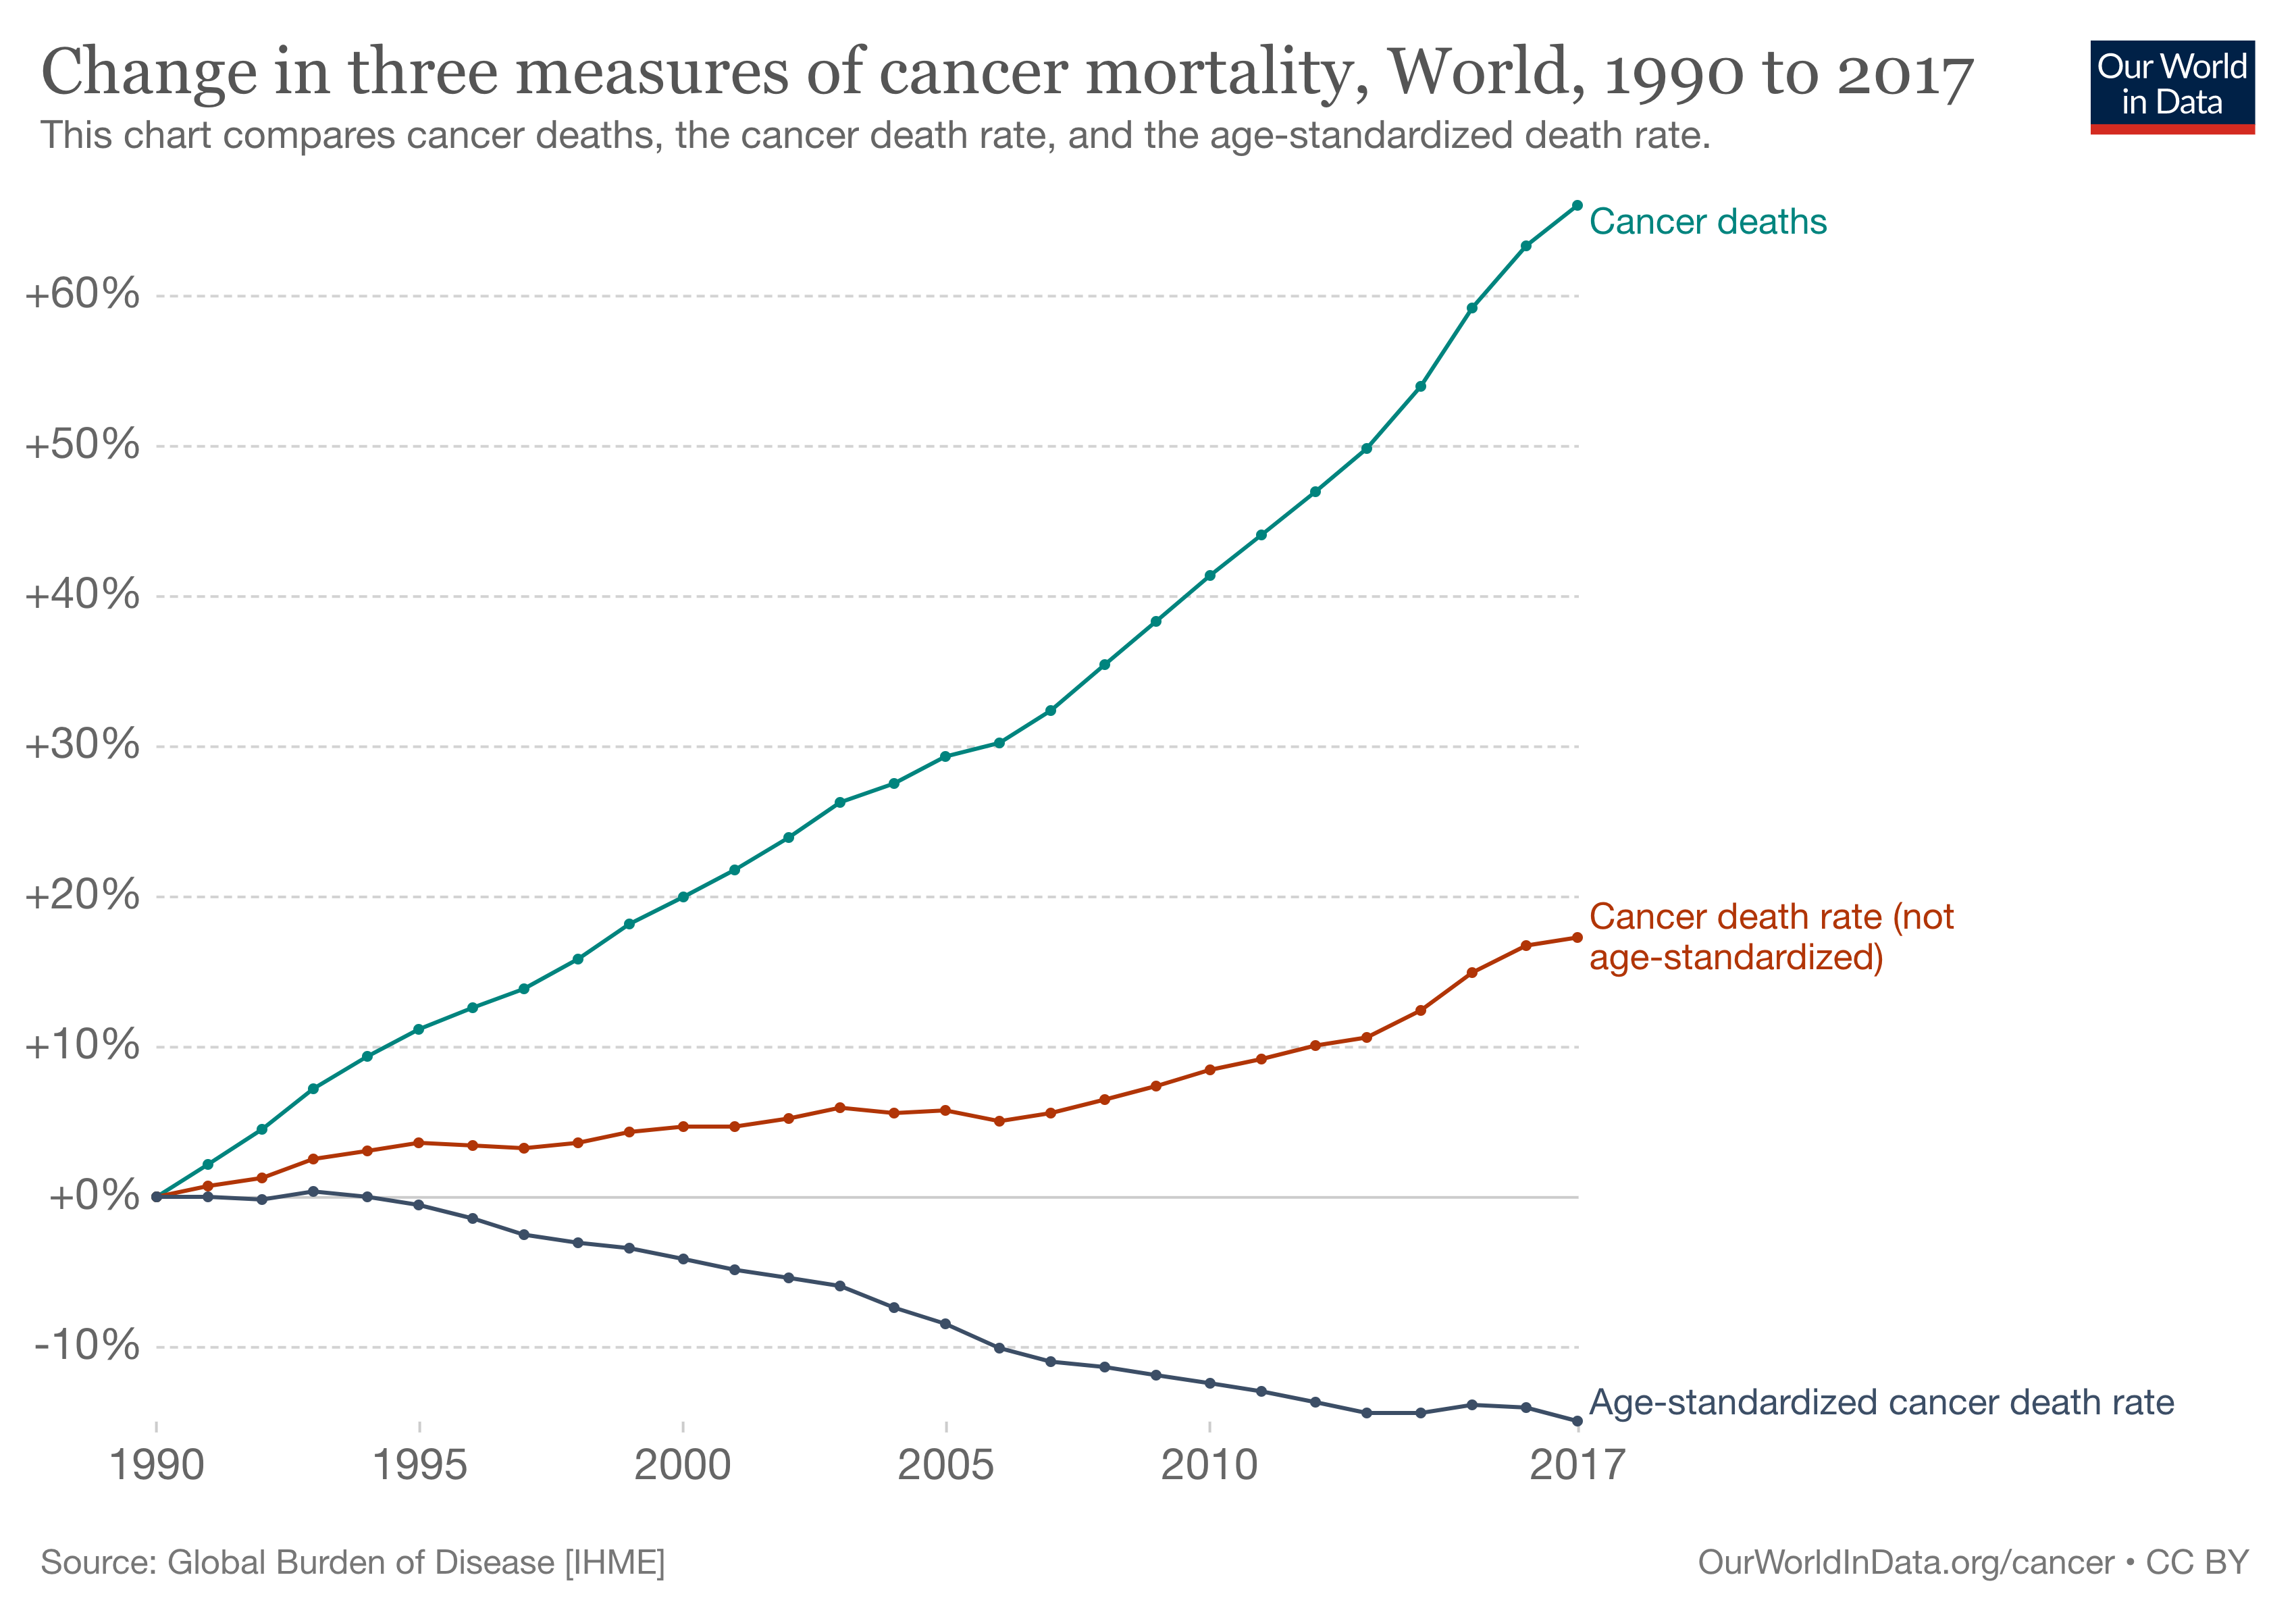
\includegraphics[width=1.0\textwidth,height=0.3\textheight,keepaspectratio]{Images/Resources/cancer-deaths-rate-and-age-standardized-rate-index.png}
      \caption{Changes in cancer mortality between 1990 and 2017. \cite{World_in_Data_undated-gc}}
      \label{fig:cancer_death}
  \end{figure}
  \FloatBarrier

  % \begin{figure}[!htb]
%     \hspace*{-1.5cm}    
%     \centering
%     \begin{subfigure}{.6\textwidth}
%         \centering
%         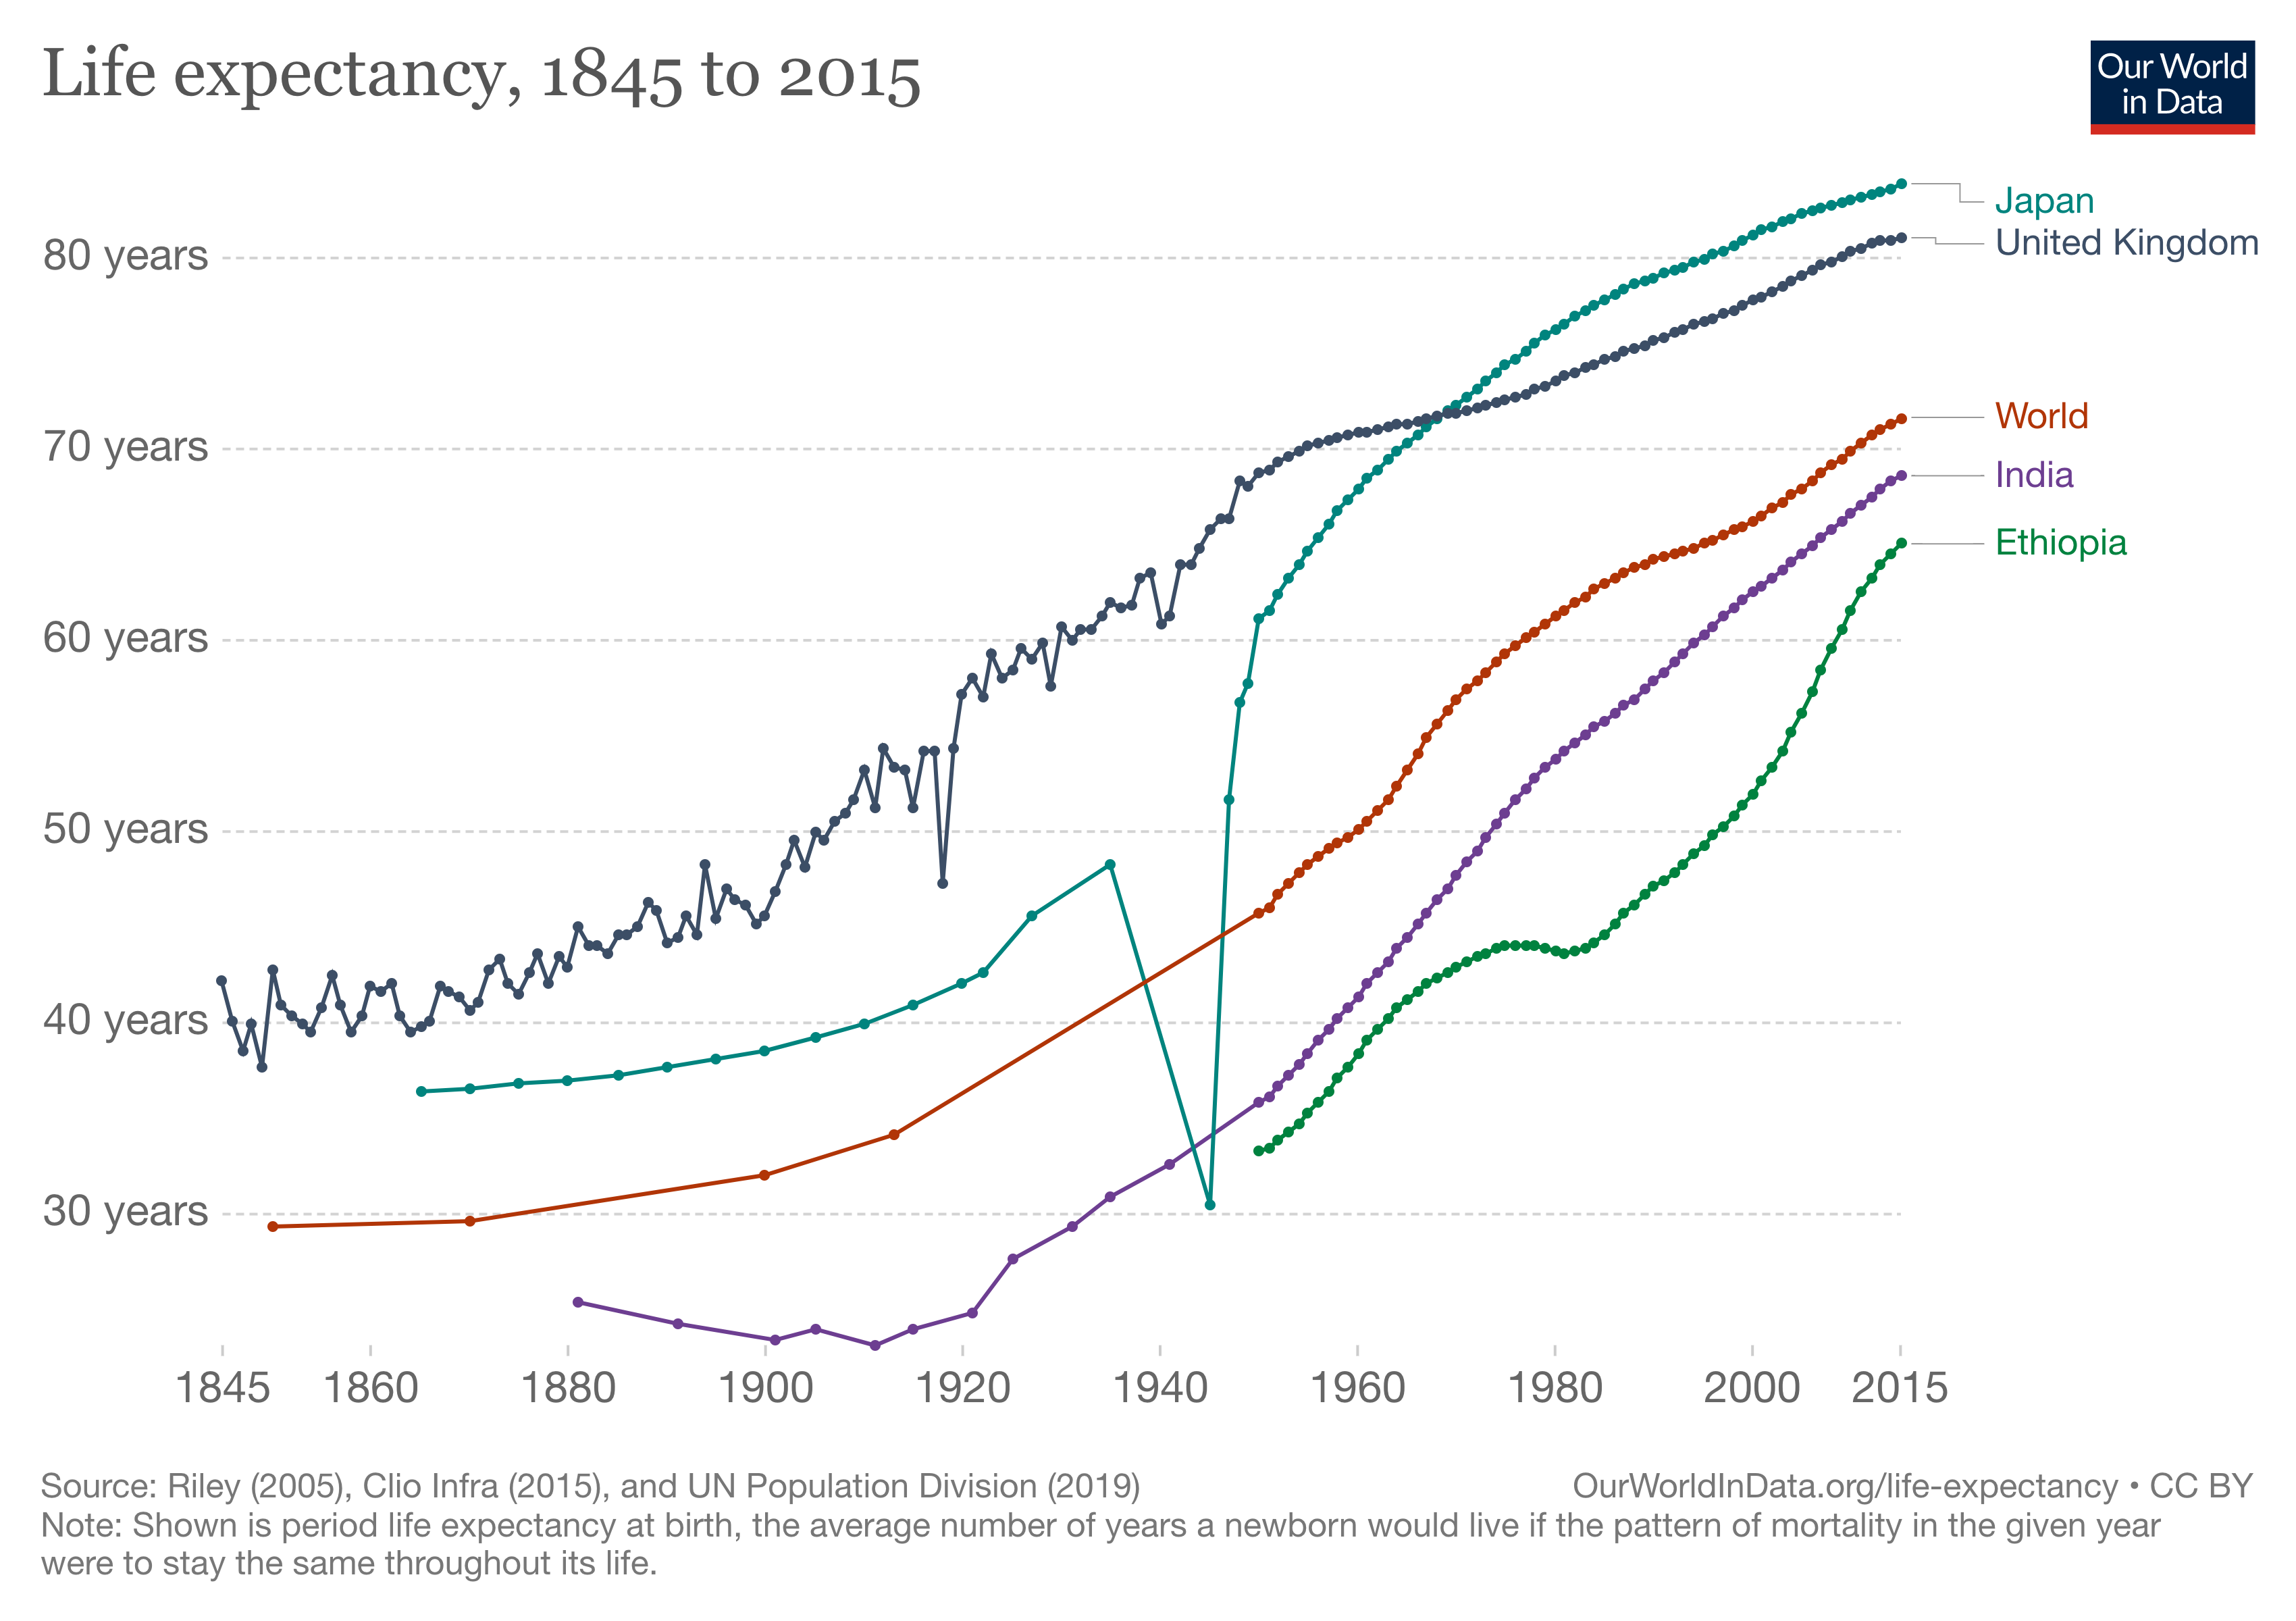
\includegraphics[width=0.8\linewidth]{Images/Resources/life-expectancy.png}
%         \caption{Life expectancy according to Our World in Data \cite{World_in_Data_undated-gc} }
%         \label{fig:life_expectancy}
%     \end{subfigure}%
%     \begin{subfigure}{.6\textwidth}
%         \centering
%         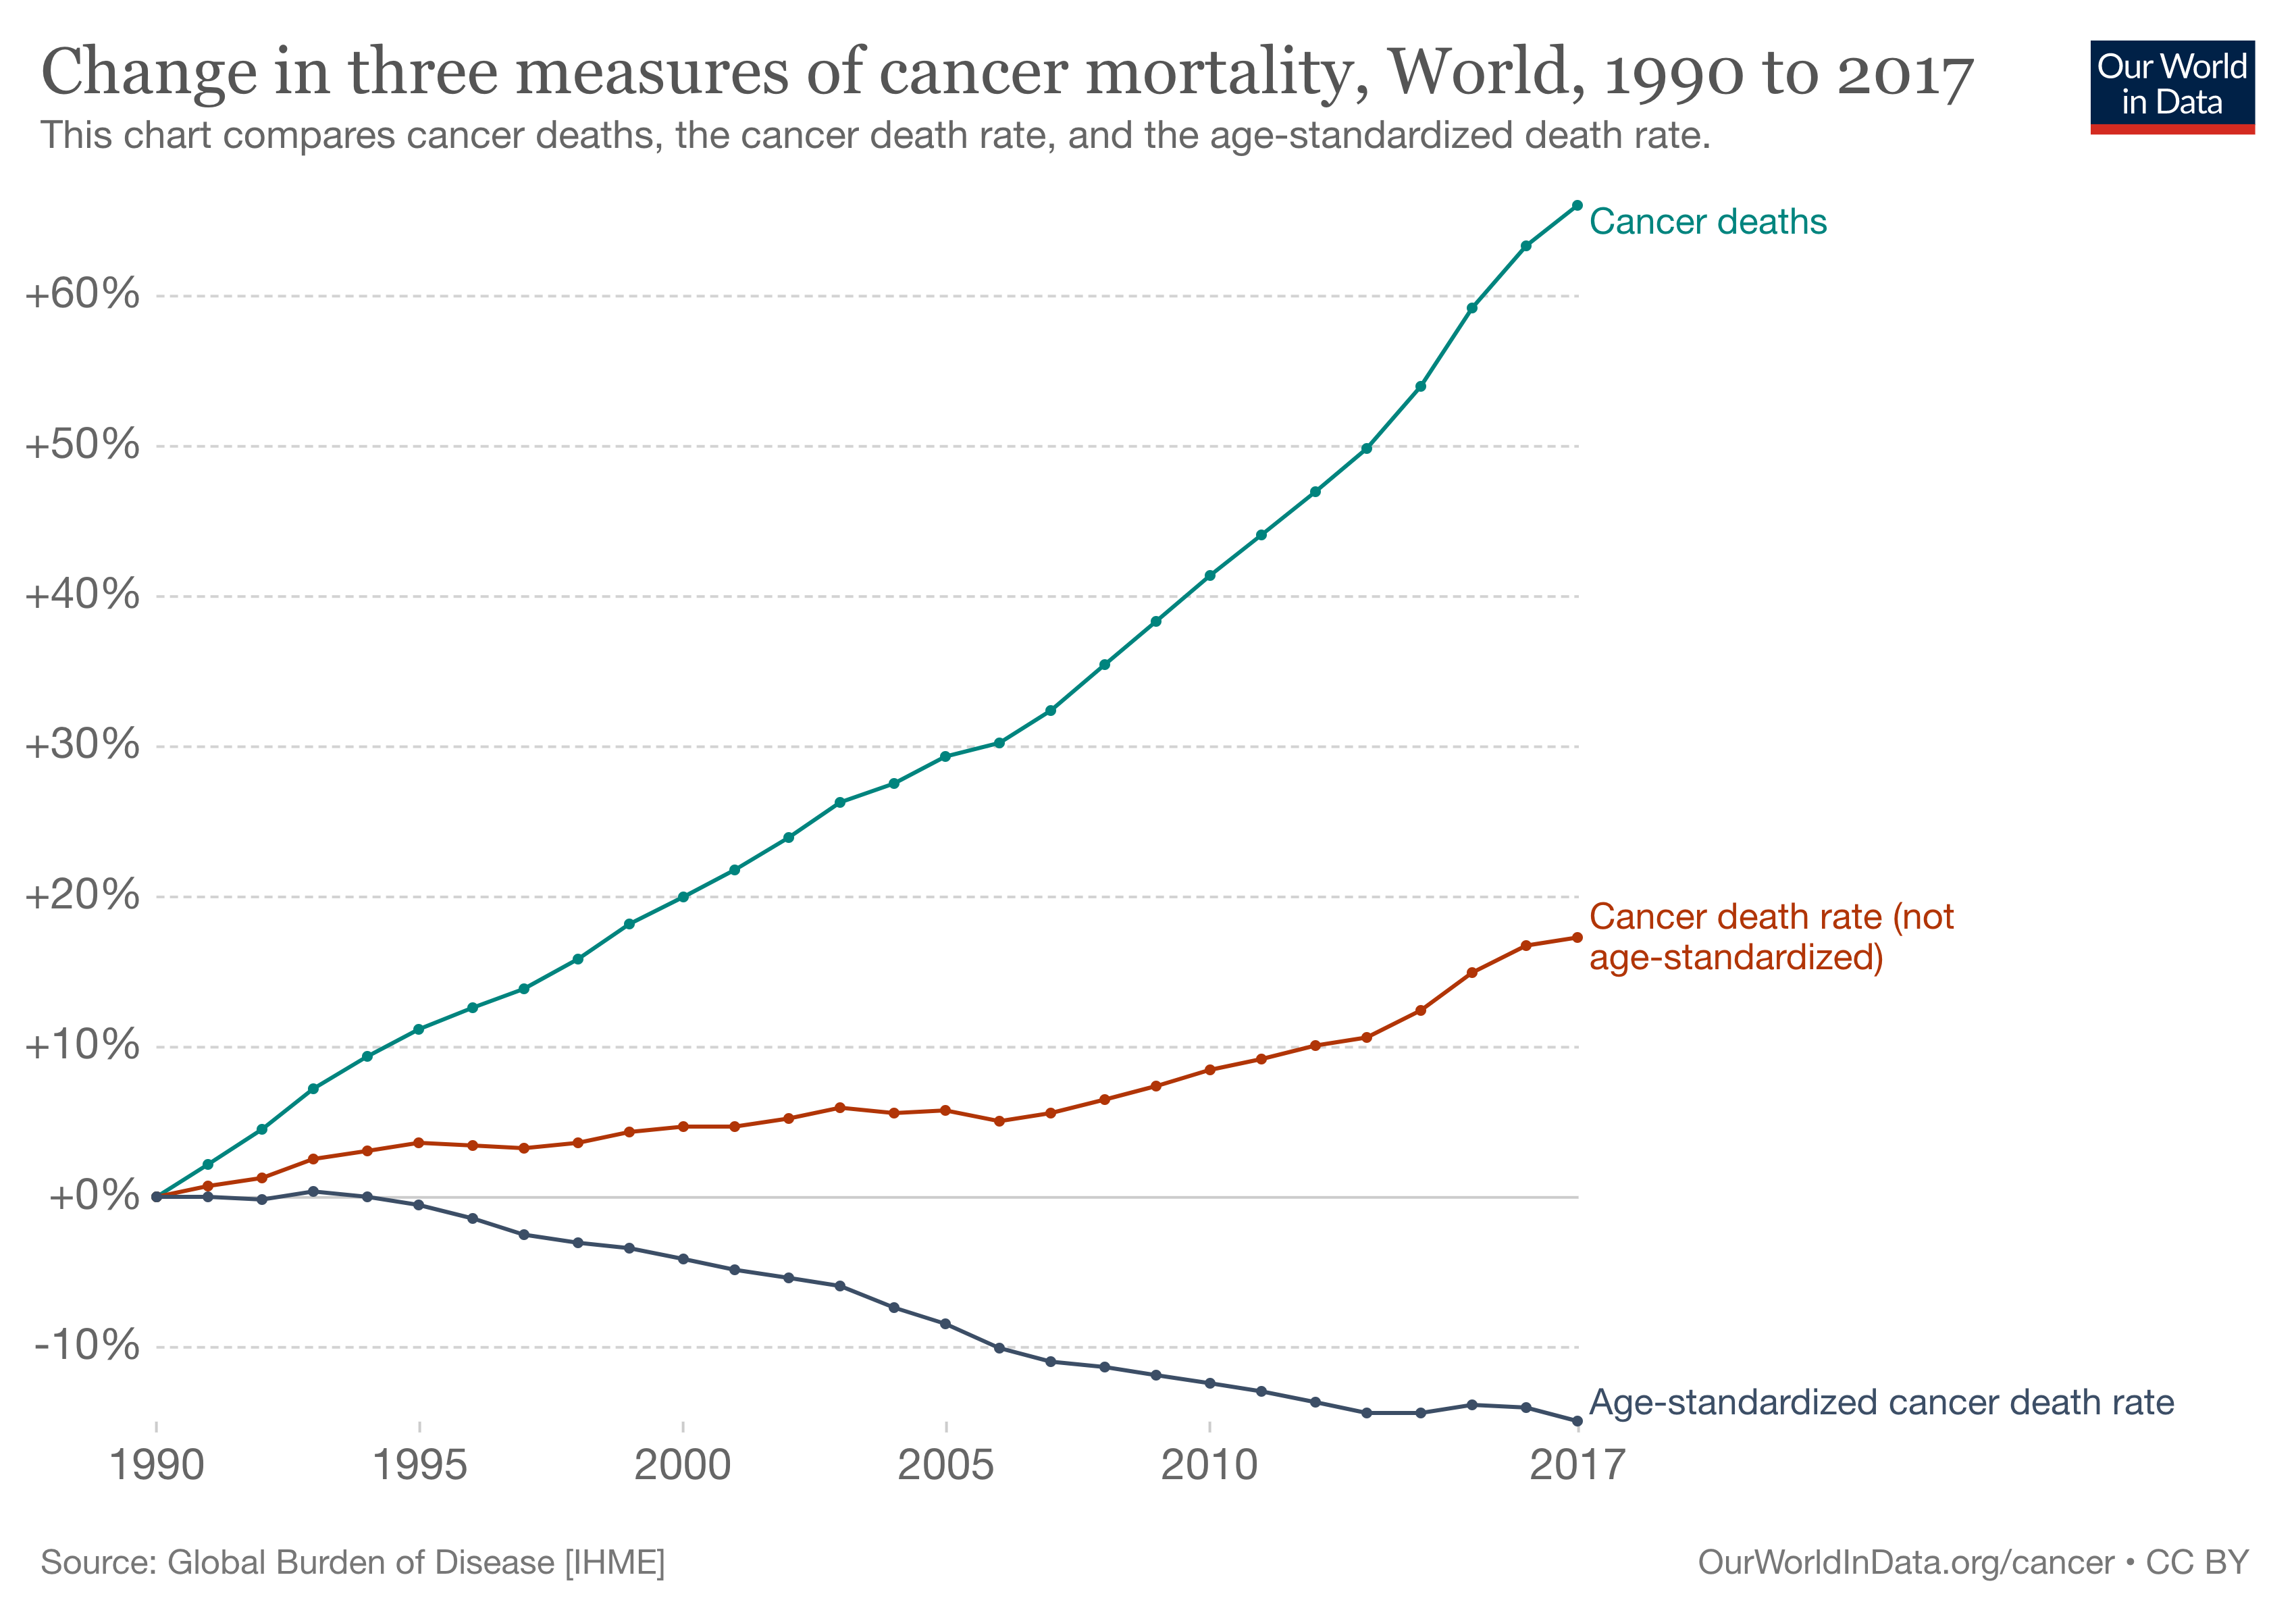
\includegraphics[width=0.8\linewidth, ]{Images/Resources/cancer-deaths-rate-and-age-standardized-rate-index.png}
%         \caption{Life expectancy according to Our World in Data \cite{World_in_Data_undated-gc}.}
%         \label{fig:cancer_death}
%     \end{subfigure}
%     \caption{Overview of the cancer and life-expectancy in modern world.}
%     \label{fig:our_world_in_data}
% \end{figure}



% \begin{figure}[!htb]
%     \centering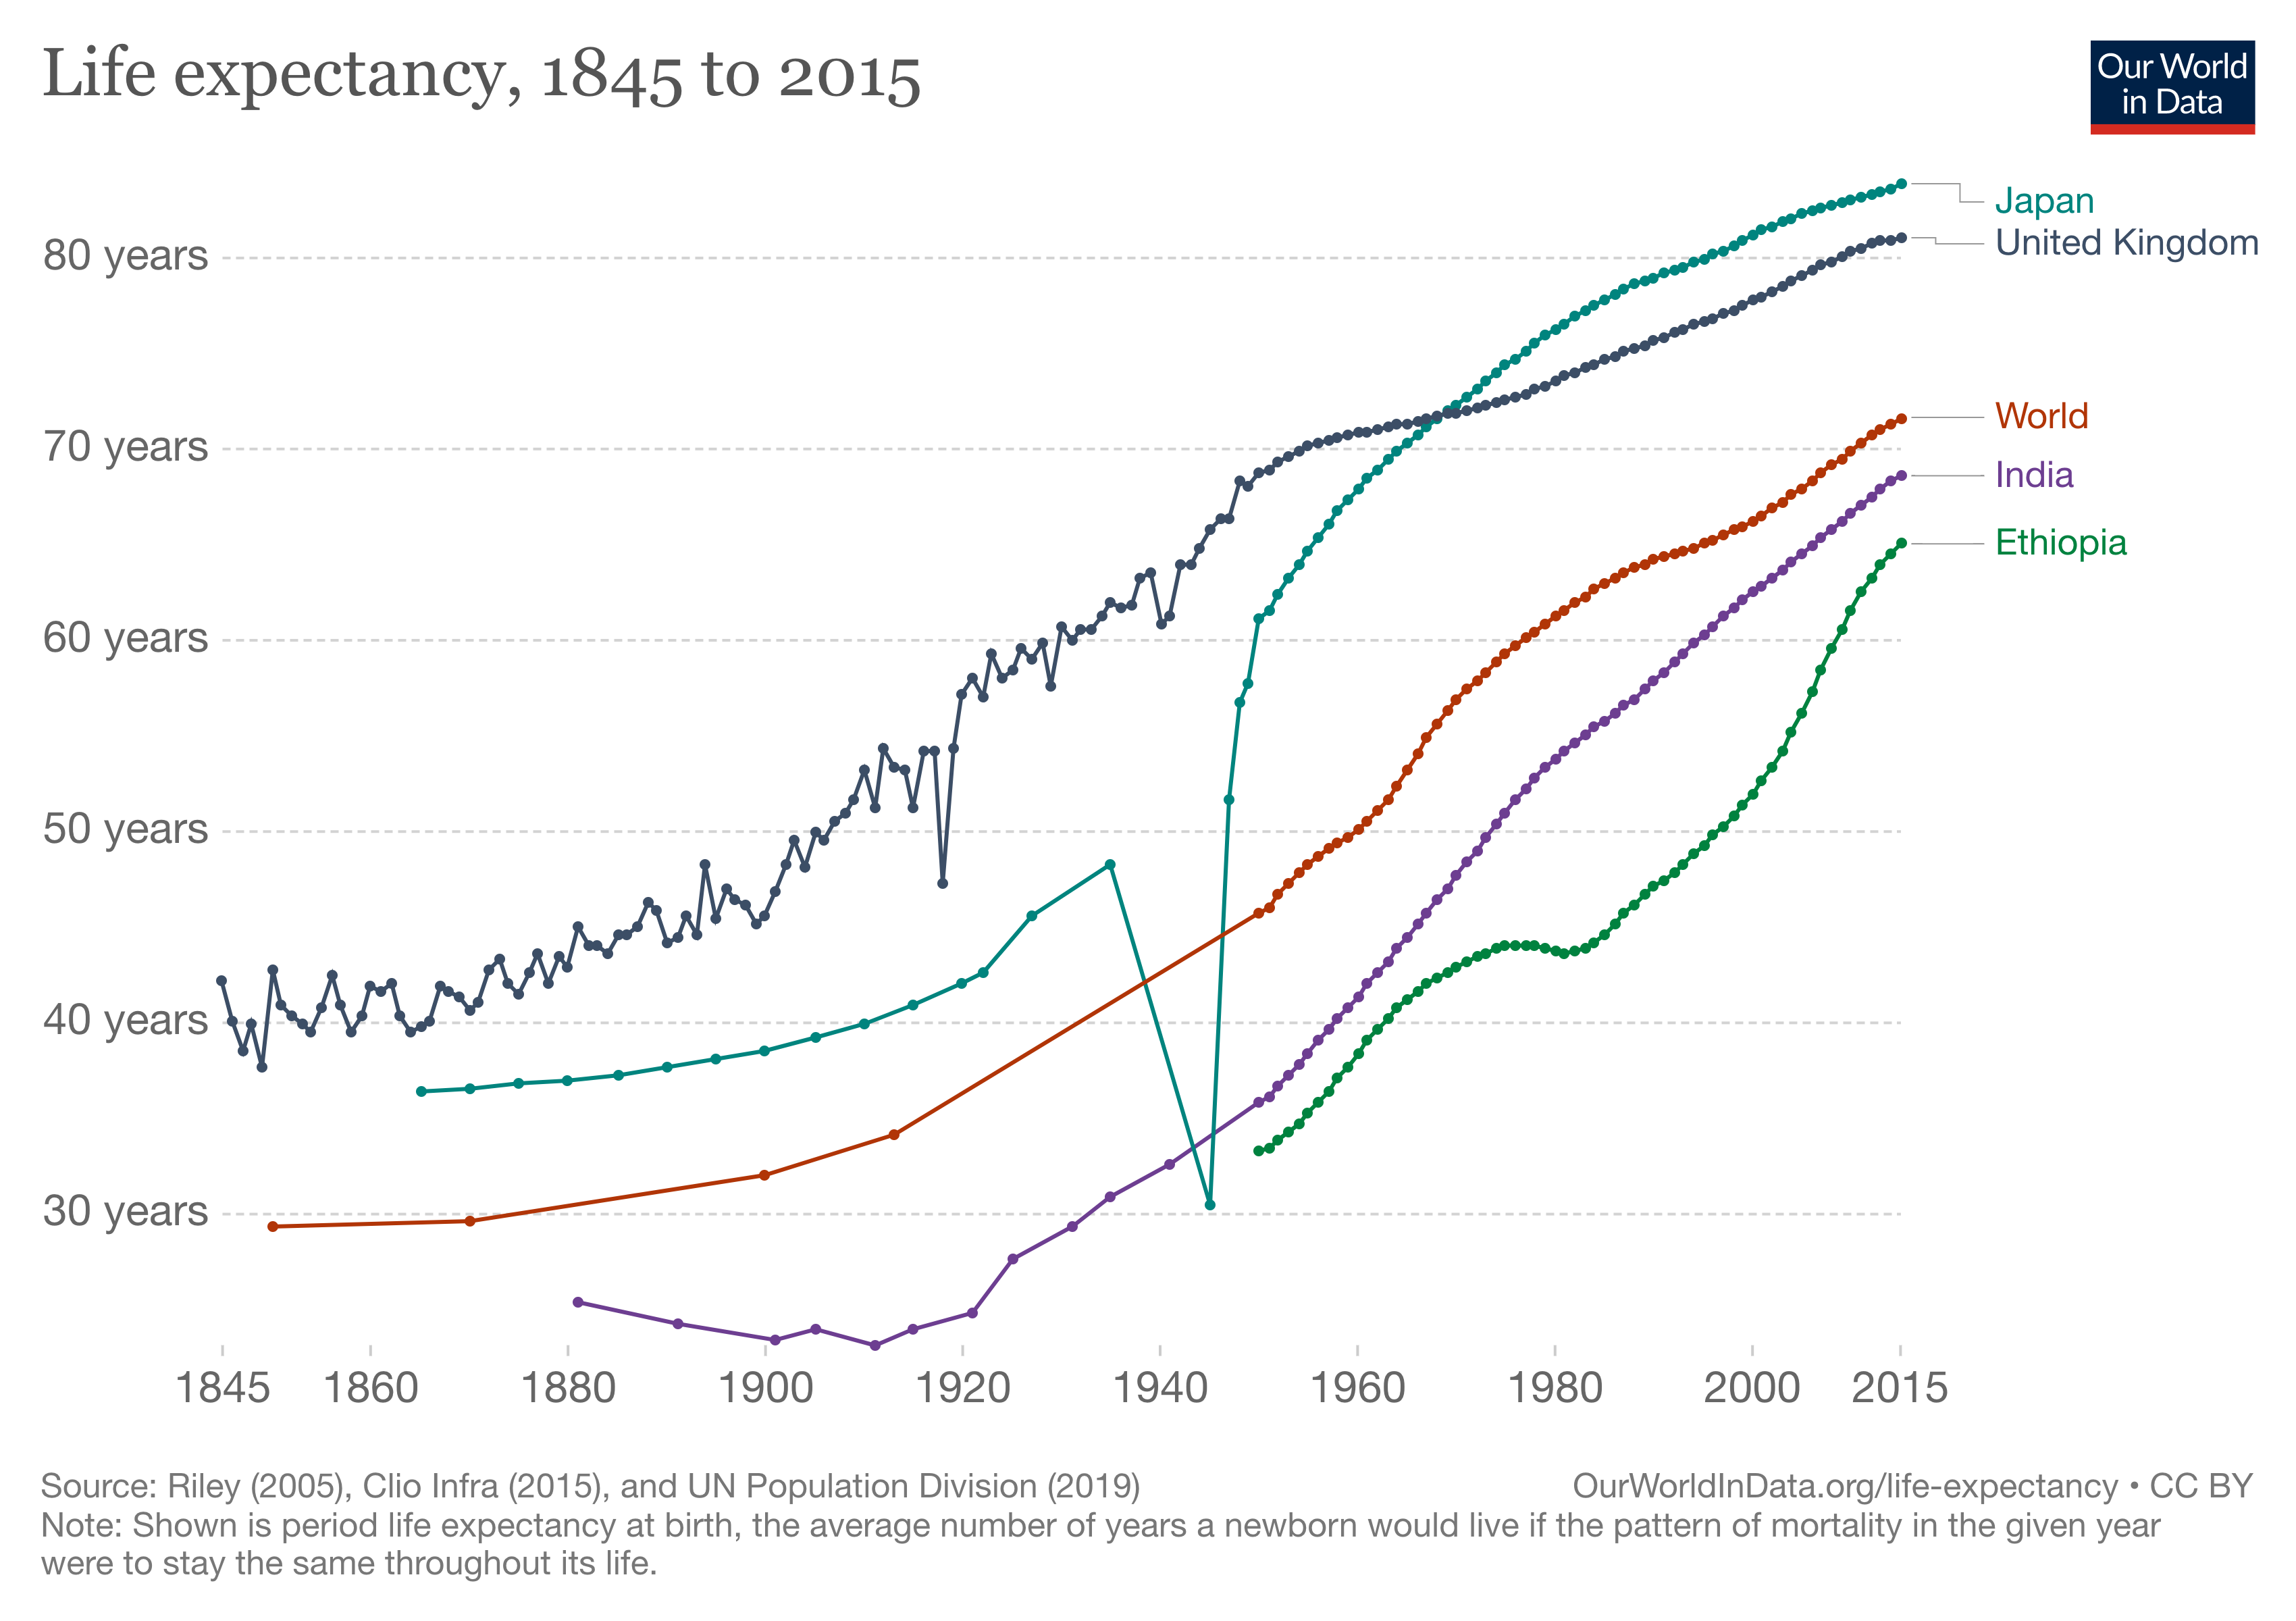
\includegraphics[width=0.8\textwidth,height=0.3\textheight,keepaspectratio]{Images/Resources/life-expectancy.png}
%       \caption{Life expectancy according to World in Data \cite{World_in_Data_undated-no}}
%       \label{fig:life_expectancy}
%   \end{figure}
%   \FloatBarrier


% \begin{figure}[!htb]
%     \centering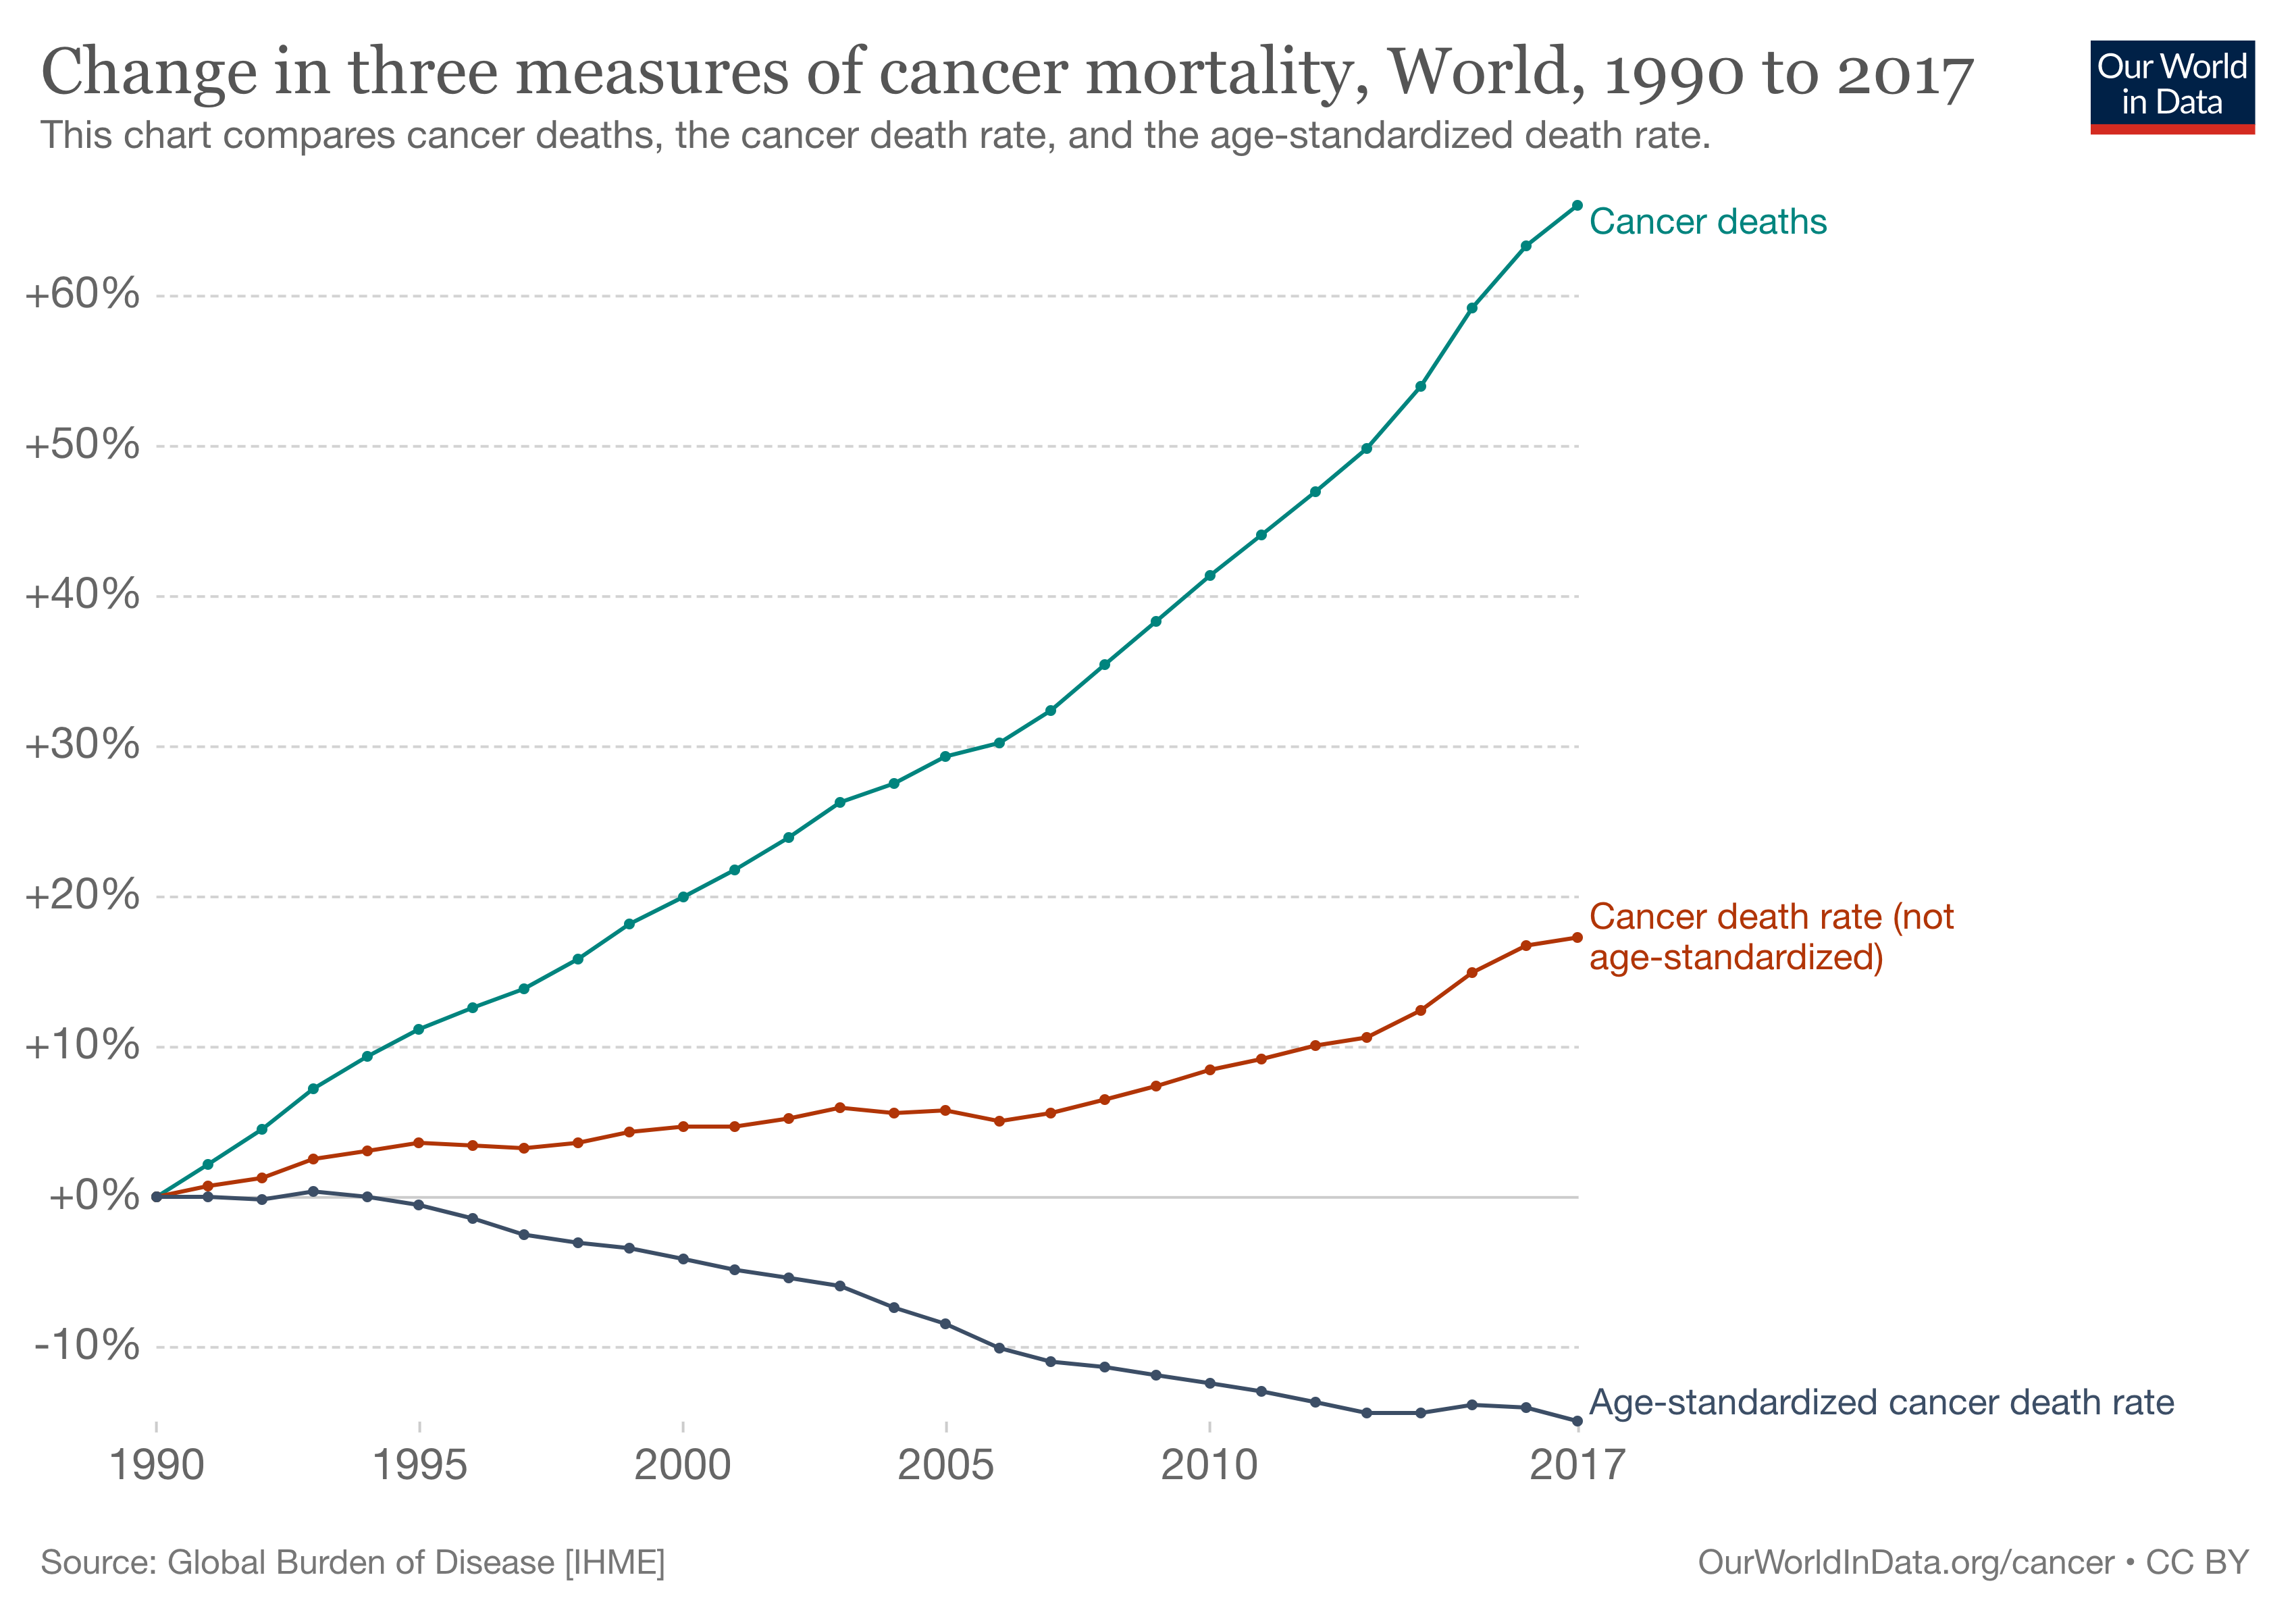
\includegraphics[width=0.8\textwidth,height=0.3\textheight,keepaspectratio]{Images/Resources/cancer-deaths-rate-and-age-standardized-rate-index.png}
%       \caption{Life expectancy according to World in Data \cite{World_in_Data_undated-gc}}
%       \label{fig:cancer_death}
%   \end{figure}
%   \FloatBarrier

